\section{РЕАЛИЗАЦИЯ CLASS-BASED WFQ В ЯДРЕ LINUX}

	\subsection{Описание устройства подсистемы планировки в ядре Linux}
	% Информация из комментариев к ним.
	% Файлы: linux/net/sched/sch_api.c, linux/include/net/{sch_generic.h,pkt_sched.h}. 

	В операционной системе Linux
	дисциплина обслуживания, обозначемая термином qdisc, используется
	для выбора пакетов из выходящей очереди для отправки на выходной интерфейс.
	Схема движения пакета приведена на Рисунке~\ref{pic:flow}. Выходная очередь
	обозначена термином egress; именно на этом этапе следования пакета
	и работает механизм qdisc.\cite{lartc}

    \begin{figure}[ht!]
        \center
        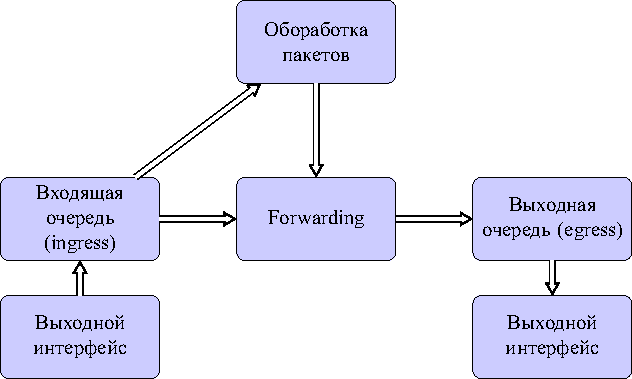
\includegraphics[scale=1.3]{pdfimages/qdisc.pdf}
        \caption{Схема движения пакета в системе Linux\cite{tcpip}}
		\label{pic:flow}
    \end{figure}

	В общем случае, дисциплина обслуживания -- это чёрный ящик, который может
	принимать поток пакетов и выпускать пакеты,
	когда устройство
	готово к отправке, в порядка и во время, определёнными спрятанным в ящике
	алгоритмом. В ядре Linux дисциплины обслуживания представляются в качестве
	модулей ядра, которые реализуют предоставляемый ядром интерфейс.

	Linux поддерживает классовые и бесклассовые дисцплины обслуживания. Примером
	бесклассовой дисциплины служит pfifo\_fast, классовой -- htb.\cite{lartc}

	Классы представляют собой одельные сущности в иерархии основной дисциплины.
	Если структура представляет собой дерево, то в классах-узлах могут содержаться
	фильтры, которые определят пакет в нужный класс-потомок. В классах-листьях
	непосредстенно располагаются очереди, которые управляются внутренней дисциплной
	обслуживания. По умолчанию это pfifo\_fast, но можно назначить другие. 

	Каждый интерфейс имеет корневую дисцплину, которой
	назначается идентификатор (handle), который используется для обращения к дисциплине.
	Этот идентификатор состоит из двух частей: мажорной (MAJ) и минорной (MIN); мажорная
	часть определяет родителя, минорная -- непосредственно класс. На Рисунке~\ref{pic:clheirh}
	представлен пример иерархии.

	\begin{figure}[ht!]
		\centering
		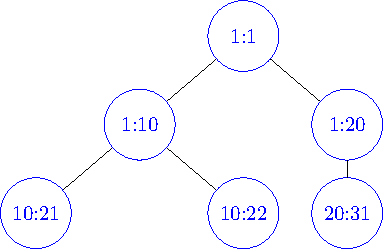
\includegraphics[scale=1.3]{./pdfimages/class_hierh.pdf}
		\caption{Схема классовой иерархии с использованием идентификаторов MAJ:MIN}
		\label{pic:clheirh}
	\end{figure}

	Идентификатор класса называется classid (к примеру, 1:10),
	а идентификтор его родителя -- parenid (1:1 для классов 1:10 и 1:20). По этим
	идентификаторам происходит поиск нужного класса внутри дисциплины.

	Такая иерархия позволяет организовать гибкую систему классификации с набором классов
	и их подклассов, пакеты в которые назначются фильтрами, которые предоставляются ядром.

	%CBWFQ является классовой дисциплиной обслуживания с конфигурируемыми классами (в отличие от
	%дисциплины PQ) и классом по умолчанию. Ядро предоставляет ряд полезных функций и структур
	%данных, которые значительно упрощают написания необходимого кода в ядре и избавляет от
	%совершения ряда критических ошибок. Таким образом, для наиболее эффективной реализации
	%дисципилны обслуживания CBWFQ следует использовать предоставляемые ядром функции.

	\subsection{Интерфейс управления трафиком}

	В Linux управление трафиком осуществляется с помощью подсистемы Traffic Control,
	которая предоставляет пользовательский интерфейс с помощью утилиты \texttt{tc}.
	\texttt{tc} -- это пользовательская программа, которая позволяет настраивать
	дисцплины обслуживания в Linux. Она использует Netlink в качестве
	коммуникационного канала для взаимодействия между пользовательским
	пространством и пространством ядра. \texttt{tc} добавляет новые дисциплины
	обслуживания, классы трафика, фильтры и предоставляет команды для
	управление всеми обозначенными объектами.\cite{tcpip}

	\texttt{tc} предоставляет интерфейс для дисцплины обслуживания,
	представленный структурой \lstinline{struct qdisc_util}, которая
	описывает функции для отправления команд и соответствующих параметров ядру
	и вывода сообщений о настройки дисциплины, списках классов и их настройки, а
	также статистику от ядра. Сообщение, помимо общей информации для подсистемы,
	содержит специфичную для дисциплины структуру с опциями, описываемую
	в заголовке ядра (pkt\_sched.h). 

	Для назначения новой дисциплины обслуживания на интерфейс используется
	команда \lstinline{tc qdisc add} системными параметрами (к примеру, название
	интерфейса), названием дисциплины и её локальными параметрами, которые
	определяются и обрабатываются в модуле дисциплины для утилиты \texttt{tc}. 
	Для внесения измнений и удаления используются соответственно \lstinline{tc change}
	и \lstinline{tc delete}.

	Для классовых дисциплин используется команда \lstinline{tc class} с подкомандами
	\lstinline{add}, \lstinline{change} и так далее. Классы обычно имеют параметры,
	отличные от параметров всей дисциплины обслуживания, поэтому нуждаются в отдельной
	структуре данных и функции обработчике.

	Таком образом, для использования дисциплины обслуживания необходимо
	реализовать интерфейс в системе \texttt{tc}. Патчи для утилиты \texttt{tc}
	и ядра Linux, обеспечивающие взаимодействие между пользовательским пространством
	и дисциплиной представлен в Приложении А. 

	\subsection{Описание интерфейса}

	API ядра для подсистемы qdisc предосавтляет две функции: \lstinline{register_qdisc(struct Qdisc_ops *ops)}
	и обратную -- \lstinline{unregister_qdisc(struct Qdisc_ops *ops)}, которые регистрируют
	и разрегистрируют дисциплину обслуживания на интерфейсе. Важно отметить, что обе эти
	функции принимают в качестве аргумента структуру \lstinline{struct Qdisc_ops},
	которая явным образом идентифицирует дисциплину обслуживания в ядре.\cite{linuxsrc}

	Структура \lstinline{struct Qdisc_ops} помимо метаинформации (в виде наименования дисциплины)
	содержит указатели на функции, которые должен реализовывать модуль дисциплины обслуживания
	для работы в ядре.\cite{linuxsrc} Если не реализовать некоторые функции,
	то ядро в некоторых случаях попробует использовать функции по умолчанию, однако
	для особенно важных (к примеру, измнение конфигурации дисциплины или класса)
	сообщит пользователю, что операция не реализована.

	Поля структуры \lstinline{Qdisc_ops} представляют собой указатели на функции 
	представленными ниже сигнатурами.
	\begin{itemize}
		\item \lstinline{enqueue}\\
   		    \lstinline{int enqueue(struct sk_buff *skb, struct Qdisc *sch, struct sk_buff **to_free);} \\
			Фукнкция добавляет пакет в очередь. Если пакет был отброшен, функция
			возращает код ошибки, говорящий о том, был отброшен пришедший пакет или
			иной, чьё место занял новый.
		\item \lstinline{dequeue}\\
			\lstinline{struct sk_buff *dequeue(struct Qdisc * sch);} \\
			Функция, возвращающая пакет из очереди на отправку. Дисциплина
			может не передавать пакет при вызове этой функции по решению
			алгоритма, в таком случае вернув нулевой указатель; 
			однако то же значение алгоритм возвращает в случае, если очередь
			пуста, поэтому в таком случае дополнительно проверяется длина
			очереди.
		\item \lstinline{peek}\\
			\lstinline{struct sk_buff *peek(struct Qdisc * sch);}\\
			Функция возвращает пакет из очереди на отправку, не удаляя его из реальной очереди,
			как это делает функция \lstinline{dequeue}.
		\item \lstinline{init}\\
			  \lstinline{int init(struct Qdisc *sch, struct nlattr *arg);}\\
			  Функция инициализирует вновь созданный экземпляр дисциплины обслуживания \texttt{sch}.
			  Вторым аргументом функции является конфигурация дисциплины обслуживния, передаваемая
			  в ядро с помощью подсистемы Netlink.
		\item \lstinline{change}\\
			  \lstinline{int change(struct Qdisc *sch, struct nlattr *arg);}\\
			  Функция изменяет текущие настройки дисциплины обслуживания. 
		\item \lstinline{dump}\\
			  \lstinline{int dump(struct Qdisc *sch, struct sk_buff *skb);}\\
			  Функция отправляет по Netlink статистику дисциплины обслуживания.
	\end{itemize}

	Также структура содержит указатель на \lstinline{struct Qdisc_class_ops},
	которая описывает указатели функции исключительно для классовых дисциплин.
	Ниже приведены наиболее важные сигнатуры и их описания.\cite{linuxsrc}
	\begin{itemize}
		\item \lstinline{find}\\
			\lstinline{unsinged long find(struct Qdisc *sch, u32 classid);}\\
			Функция возвращает приведённый к \lstinline{unsinged long} адресс класса по его идентификатору (\lstinline{classid}).
		\item \lstinline{change} \\
			\lstinline{int change(struct Qdisc *sch, u32 classid, u32 parentid, struct nlattr *attr, unsinged long *arg);}\\
			Функция используется для изменения и добавления новых классов в иерархию классов. 
		\item \lstinline{tcf_block}, \lstinline{bind_tcf}, \lstinline{unbind_tcf}\\
			В данном случае, описание сигнатур не даст какой-либо значимой информации; практически
			для всех дисциплин обслуживания они идентичны. Эти функции предназначаются для работы
			системы фильтрации.
		\item \lstinline{dump_class}\\
			\lstinline{int dump_class(struct Qdisc *sch, unsinged long cl, struct sk_buff *skb, struct tcmsg *tcm);} \\
			Функция предназначается для передачи по Netlink информации о классе и дополнительной статистики, собранной
			во время функционирования класса.
	\end{itemize}

	Для классовых дисцплин, помимо описанного, реализуют классификацию пакетов, которая
	определяет класс, куда попадёт пакет. Классификация обычно выражается в функции \lstinline{classify},
	которая вызывается при добавлении пакета в очередь (функция \lstinline{enqueue}) определяет, какому классу
	 принадлежит пакет, и возвращает указатель на этот класс.
	Экземпляр структур для дисциплины обслуживания CBWFQ приведён в патче, представленном в Приложении B.

	\subsection{Алгоритм CBWFQ}

		Реализация CBWFQ требует:
		\begin{itemize}
			\item вычисление виртуального времени окончания обслуживания для каждого
				   пакета в очередях, как этого требует WFQ;
			%\item поддержку приоритетной структуры данных для хранения пакетов,
			%	  чтобы возвращать пакет с минимальным виртуальным временем
			%	  окончания обслуживания; 
			\item поддержку классов и классовых операций;
			\item фильтрацию для классификации трафика по классам.
		\end{itemize}

		

%
%		\subsubsection{Структуры хранения данных Class-Based WFQ}
%	
%			Обычно классовые дисциплины обслуживания содержат две основные структуры:
%			для описания непосредственно дисцилины и для описания класса.  
%			Структура дисциплины содержит в себе данные, которые описывают всю дисциплину:
%			это могут быть структура данных с классми (в виде списка или дерева),
%			ограничения на очереди, статистика по всей дисциплине и так далее.
%			Структура класса, соответственно, содержит непосредственно очередь и описывающие
%			класс параметры.
%
%			Для функционирования WFQ каждый класс должен содержат в себе вес.
%			В ядре Linux для того, чтобы оперировать числами с плавающей точкой, нужно
%			использовать специальные функции, которые позволяют использовать модуль
%			операций с плавающей точкой (Float Point Unit, FPU); это вычислительно
%			дорогая операция, поэтому алгоритм был изменён таким образом, чтобы
%			использовались целочисленные значения. Поэтому веса хранятся в процентах.
%
%			Определение структур представлено в Приложении B. 
%
%
%		\subsubsection{Вычисление виртуального времени}
%			\begin{algorithmic}
%				\Function{eval\_finish\_time}{Q, c, pkt}
%					\State {// Если очередь была пуста (т.е. не была активна), время сбрасывается в 0.}
%					\State s $\gets$ 0
%					\State {// Сумма весов активных очередей.}
%					\State active\_w $\gets$ ACTIVE\_WEIGHTS(Q)
%					\If {c.queue is not empty $\land$ active\_w $\neq$ 0}
%						\State {//Вычисляем виртуальное время от начала обработки.}
%        				\State {// В ядре вычисления с плавающей запятой затруднены,}
%        				\State {// из-за чего стараемся изменить вычисления так, чтобы их избегать.}
%						\State va $\gets \dfrac {(\text{pkt.arrive\_time} - \text{c.prev\_ft}) \cdot 100} {\text{active\_w}}$ 
%        				\State {// Вычисление времени начала обработки.}
%        				\State s $\gets$ MAX(c.prev\_ft, va)
%					\EndIf
%    				\State \Return s $ + \dfrac {\text{pkt.len} \cdot 100} {\text{c.weight}}$
%				\EndFunction
%			\end{algorithmic}
%
%		\subsubsection{Добавление пакета в очередь}
%
%			Алгоритм добавления пакета обычно состоит из схожих действий:
%			классификация и добавление в очередь, если есть место в очереди
%			для пакета. 
%
%			\begin{algorithmic}
%				\Function{enqueue}{Q, pkt}
%					\State {// Сначала нужно классифицировать пакет в очередь.}
%					\State {// Функция классификации определяет очередь, которой}
%					\State {// соответствует пакет, с помощью заданных фильтров}
%					\State {// и возвращает указатель на класс.}
%					\State c $\gets $ CLASSIFY(Q, pkt)
%					\State {// Отбрасываем пакет, если длина очереди достигла предела.}
%					\If {c.queue\_len < c.limit}
%						\State DROP(Q, pkt)
%					\ElsIf {\Call{q.enqueue}{pkt}}
%    					\State {// Ради экономии ресурсов, храним два виртуальных времени:}
%    					\State {// текущего и прошлого пакета; и считаем время только для}
%    					\State {// пакета, который пришёл в пустую очередь}
%    					\If {c.queue is empty}
%							\State c.prev\_ft $\gets$ c.ft
%							\State c.ft $\gets$ EVAL\_FINISH\_TIME(Q, c, pkt)
%    					\EndIf
%					\EndIf
%				\EndFunction
%			\end{algorithmic}
%
%			Специфичным добавлением CBWFQ является вычисление времени конца обработки.
%			Оно вычисляется каждый раз, когда пакет добавляется в пустую очередь.
%			Это сделано, чтобы не реализовывать дополнительные структуры для
%			хранения и тем самым тратить меньше ресурсов.
%
%		\subsubsection{Удаление пакета из очереди}
%
%			Функция удаления пакета из очереди непосредственно реализует
%			планировщик WFQ.
%
%			\begin{algorithmic}
%				\Function{dequeue}{Q}
%					\State {// Находим класс с наименьшим финальным временем.}
%					\State {// Реализуется это простым простым прохождением по списку}
%					\State {// классов.}
%					\State C $\gets$ FIND\_MIN\_FT(Q)
%					\State {// Если не найдено классов, то все очереди пусты.}
%					\If {C is null}
%						\State \Return null
%					\EndIf
%					\State pkt $\gets$ C.QUEUE.DEQUEUE(C.queue)
%					\State {// Вычисляем новое финальное время для следующего пакета}
%					\State pkt\_next $\gets$ C.QUEUE.PEEK(C.queue)
%					\State C.ft $\gets$ EVAL\_FINISH\_TIME(Q, C, pkt\_next)
%					\State \Return pkt 
%				\EndFunction
%			\end{algorithmic}
